% ********** BEGIN Chapter 3 **********
\chapter{Background Study}
\label{sec:BackgroundStudy}

\section{VoIP Market}
\label{sec:BackgroundStudy:VoIPMarket}


\subsection{VoIP Service Provider}
\label{sec:BackgroundStudy:VoIPMarket}

\subsection{VoIP Client}

\subsection{Solution Provider}



\section{Third Party Call Control}

In the traditional telephony context, third party call control allows one entity (which we call the controller) to set up and manage a communications relationship between two or ore other parties.  Third party call control (referred to as \textbf{3pcc}\label{sym:3pcc}) is often used for operator
services (where an operator creates a call that connects two participants together) and conferencing.\cite{RFC3725}

\begin{figure}
\centering
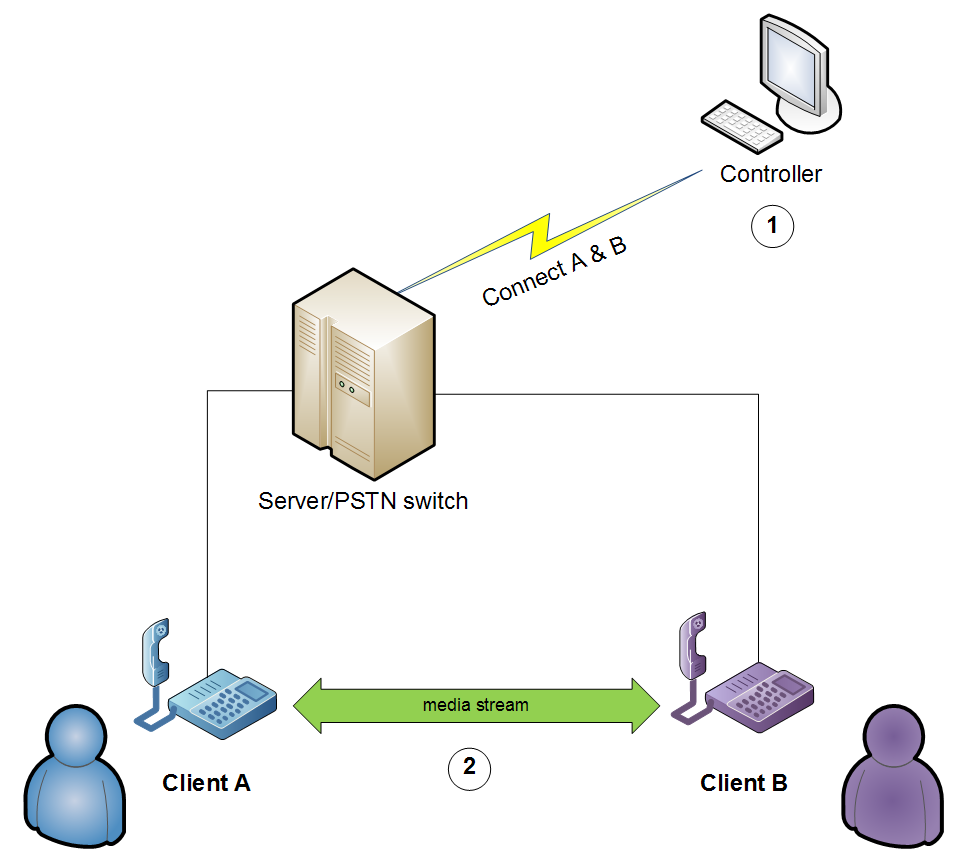
\epsfig{file=chap03/resources/3pcc, width=4in}
\caption{Third party call control}
\end{figure}

% ********** End of chapter 3 **********
